% ju 18-Feb-24 Mars-Rover.tex
\documentclass{vorlage-design-main}
\usepackage[utf8]{inputenc}
\usepackage{longtable}
\usepackage{blindtext,alltt}
%% Ganze Überschrift
\title{Thema}

%% Kürzerer Titel zur Verwendung im Seitenkopf
\runningtitle{Kurztitel}
\author{Jan Unger}
% \author{2.}
\date{\today}

%% Die .bib-Datei mit vollständigen Referenzen zur Verwendung mit biblatex. articleclass lädt das Paket biblatex-chicago mit Anpassungen
\addbibresource{literatur.bib}

\begin{document}

\maketitle

\begin{abstract}

\end{abstract}

\begin{figure}
\centering
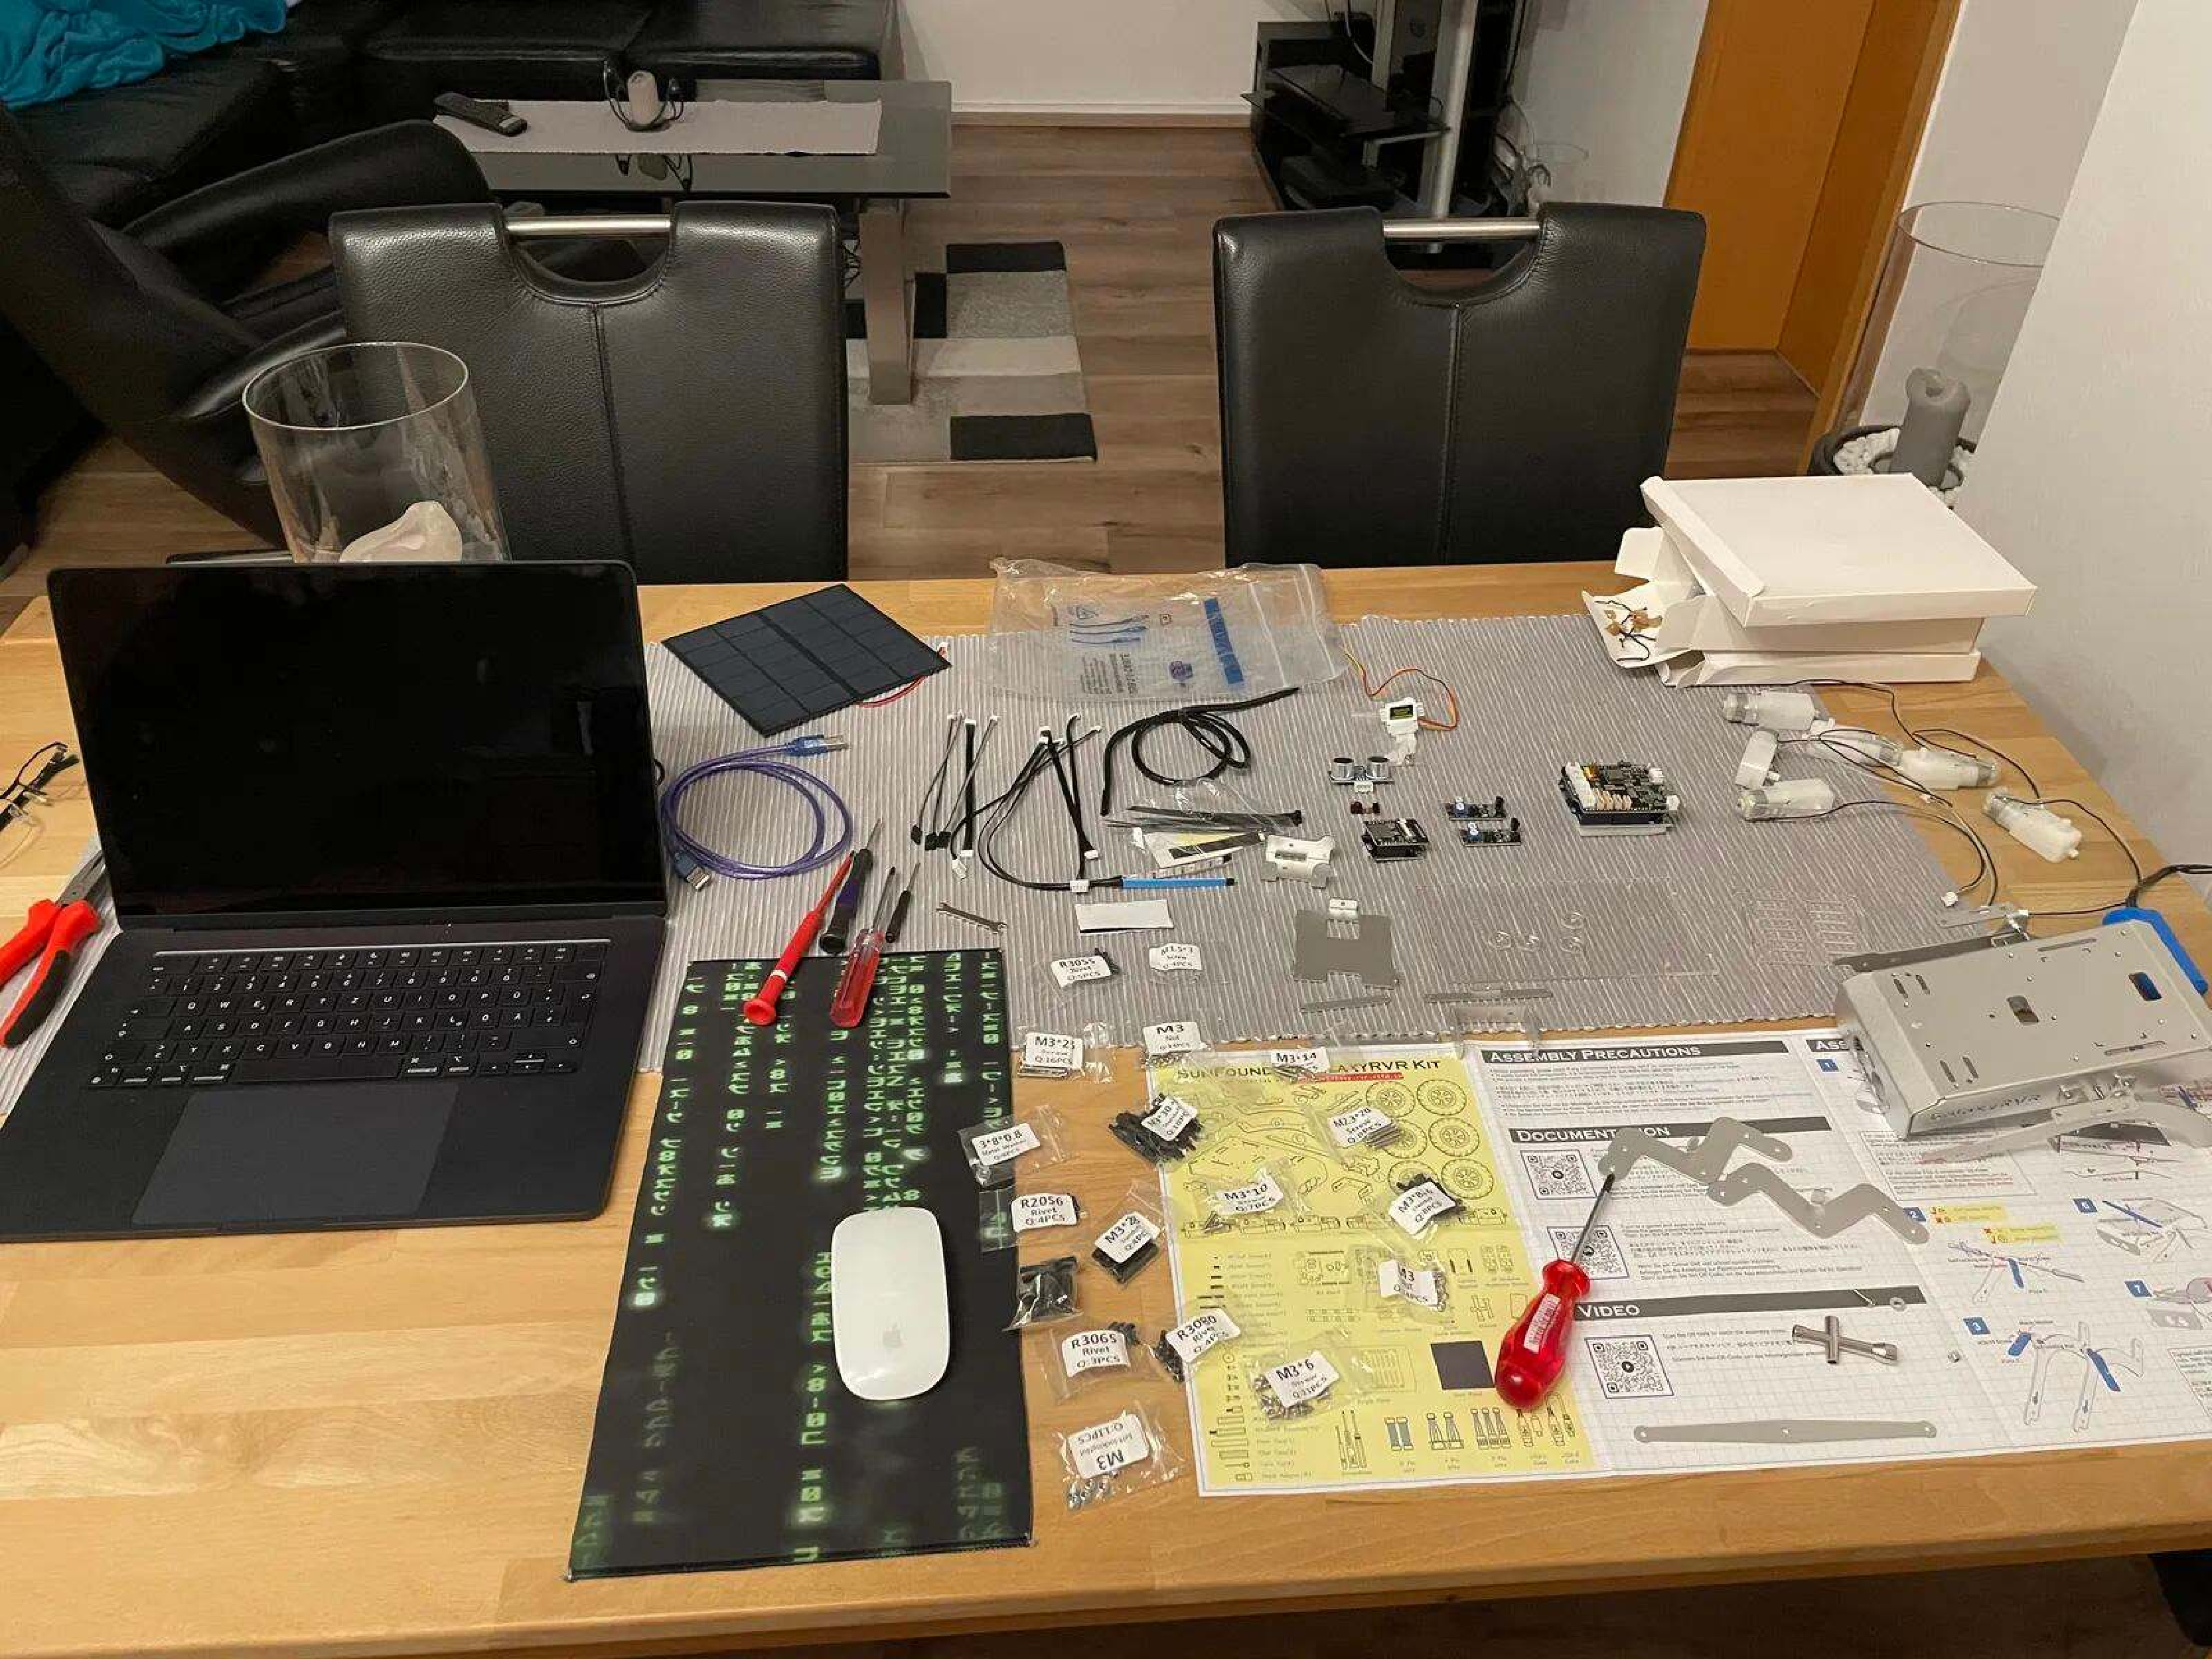
\includegraphics[width=0.8\textwidth]{images/rover-bau.pdf}
\floatnotes{}
%\label{fig:}
\caption{Mars-Rover Montage}
\end{figure}

\begin{figure}
\centering
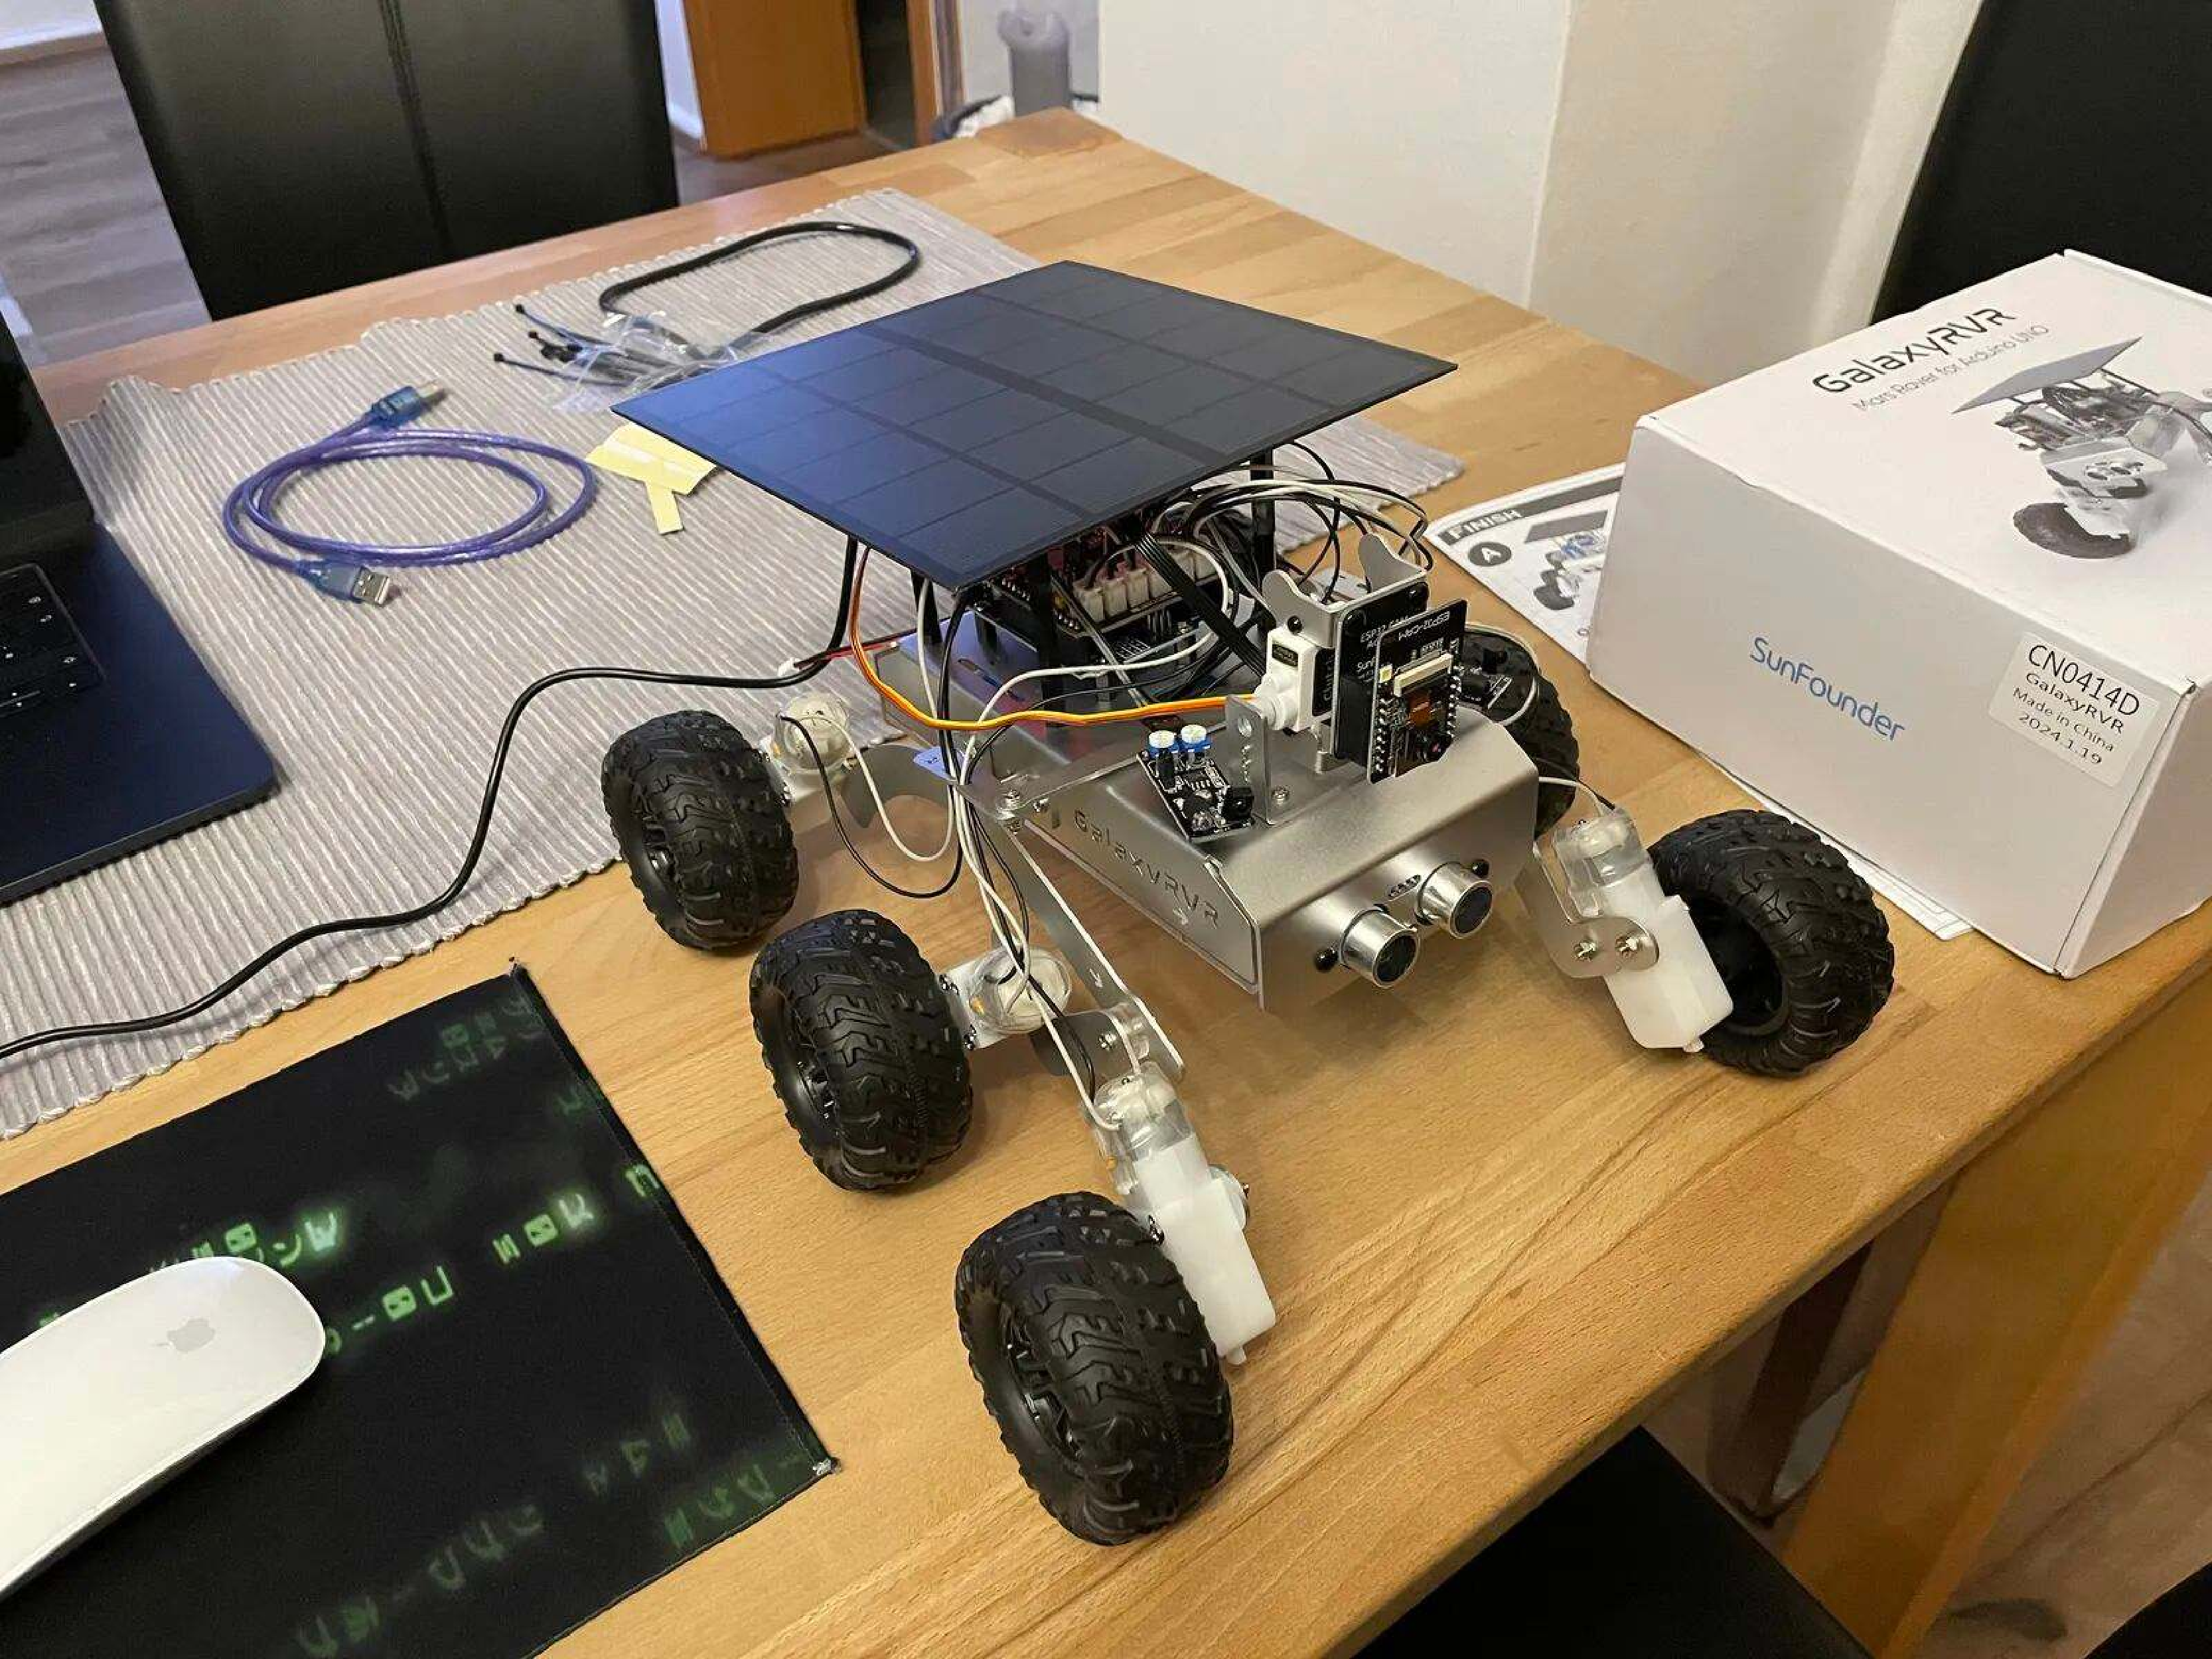
\includegraphics[width=0.8\textwidth]{images/rover-bau2.pdf}
\floatnotes{}
%\label{fig:}
\caption{Mars-Rover Montage 2}
\end{figure}

\hypertarget{enthuxfcllung-des-mars-rovers}{%
\subsection{Enthüllung des
Mars-Rovers}\label{enthuellung-des-mars-rovers}}

\hypertarget{unterschiede-in-den-designs}{%
\subsubsection{Unterschiede in den
Designs}\label{unterschiede-in-den-designs}}

\begin{itemize}

\item
  \textbf{Sojourner (1997)}: Als erster Rover auf dem Mars klein und
  relativ einfach gestaltet, mit dem Hauptziel, die Machbarkeit der
  Rover-Technologie auf dem Mars zu demonstrieren.
\item
  \textbf{Spirit und Opportunity (2004)}: Beide hatten ein
  ausgeklügelteres Design als Sojourner, waren größer, hatten eine
  längere Missionsdauer und waren mit fortschrittlicheren
  wissenschaftlichen Instrumenten ausgestattet, um Geologie und
  Atmosphäre zu erforschen.
\item
  \textbf{Curiosity (2012)}: Noch größer und komplexer, mit einem Labor
  an Bord, um chemische Analysen durchzuführen und nach Bedingungen für
  mikrobielles Leben zu suchen.
\item
  \textbf{Perseverance (2021)}: Baut auf Curiositys Design auf, mit
  zusätzlichen Instrumenten für astrobiologische Forschung,
  einschließlich der Suche nach fossilen Mikroben, und dem
  experimentellen Mars-Hubschrauber Ingenuity.
\end{itemize}

\hypertarget{gemeinsamkeiten}{%
\subsubsection{Gemeinsamkeiten}\label{gemeinsamkeiten}}

\begin{itemize}

\item
  Alle Rover sind mit Kameras und wissenschaftlichen Instrumenten
  ausgestattet, um den Mars zu studieren.
\item
  Solarenergie (bis Curiosity, der mit einem Radioisotopengenerator
  betrieben wird) und Kommunikationsfähigkeit mit der Erde.
\item
  Mobilität auf der Oberfläche zur Durchführung geologischer
  Untersuchungen und Atmosphärenmessungen.
\end{itemize}

\hypertarget{einfluss-der-missionsziele-auf-das-design}{%
\subsubsection{Einfluss der Missionsziele auf das
Design}\label{einfluss-der-missionsziele-auf-das-design}}

\begin{itemize}

\item
  Mit jedem Rover wuchsen die Missionsziele, was zu komplexeren Designs
  führte. Während Sojourner hauptsächlich die Technologie testete,
  suchten spätere Rover nach Wasserzeichen, aktuellen und vergangenen
  Lebensbedingungen und bereiteten die Mars-Erkundung durch Menschen
  vor.
\item
  Die Instrumentenauswahl reflektiert die spezifischen
  wissenschaftlichen Ziele jeder Mission.
\end{itemize}

\hypertarget{technologische-fortschritte}{%
\subsubsection{Technologische
Fortschritte}\label{technologische-fortschritte}}

\begin{itemize}

\item
  Fortschritte in der Robotik, Navigation, Energieversorgung und
  wissenschaftlichen Instrumentierung.
\item
  Von einfachen Kameras und Analyseinstrumenten zu hochauflösenden
  Kamerasystemen, Umweltsensoren, chemischen Analyseinstrumenten und dem
  ersten Fluggerät (Ingenuity).
\end{itemize}

\hypertarget{vorschluxe4ge-fuxfcr-den-nuxe4chsten-mars-rover}{%
\subsubsection{Vorschläge für den nächsten
Mars-Rover}\label{vorschlaege-fuer-den-naechsten-mars-rover}}

\begin{itemize}

\item
  Erweiterte Lebenssuche: Noch spezifischere Instrumente zur Detektion
  von Leben oder organischen Molekülen.
\item
  Probe-Return-Technologie: Integration von Systemen, um Proben für eine
  zukünftige Rückkehr zur Erde zu sammeln und zu konservieren.
\item
  Autonomie: Verbesserte autonome Navigationssysteme, um mehr Terrain
  sicher und effizient zu erkunden.
\item
  Technologien zur Unterstützung menschlicher Exploration: Experimente
  zur Ressourcengewinnung aus der Marsatmosphäre oder dem Boden.
\end{itemize}

\hypertarget{reflexionen-und-fragen}{%
\subsubsection{Reflexionen und Fragen}\label{reflexionen-und-fragen}}

\begin{itemize}

\item
  Wie können zukünftige Rover zur Vorbereitung menschlicher Missionen
  auf den Mars beitragen?
\item
  Welche neuen Technologien könnten zukünftige Rover revolutionieren?
\item
  Inwiefern können die gesammelten Daten dazu beitragen, die
  langfristige Bewohnbarkeit des Mars für Menschen zu verstehen?
\end{itemize}

\hypertarget{verstuxe4ndnis-und-bau-des-rocker-bogie-systems}{%
\subsection{Verständnis und Bau des
Rocker-Bogie-Systems}\label{verstaendnis-und-bau-des-rocker-bogie-systems}}

\begin{itemize}

\item
  \textbf{Einführung in das Rocker-Bogie-System}: Ein Federungssystem,
  das bei allen Mars-Rovern von Sojourner bis Perseverance verwendet
  wird, um eine optimale Anpassung an das raue Marsgelände zu
  gewährleisten.
\end{itemize}

\hypertarget{schritt-1-rocker-bogie-systems}{%
\subsubsection{Schritt 1:
Rocker-Bogie-Systems}\label{schritt-1-rocker-bogie-systems}}

\begin{itemize}

\item
  Das Rocker-Bogie-System ermöglicht es, dass alle Räder trotz unebener
  Oberflächen Bodenkontakt halten.
\item
  Zwei Hauptteile: >>Rocker<< (große Gliedmaßen für Bodenkontakt) und
  >>Bogie<< (kleineres Verbindungssystem für Flexibilität).
\end{itemize}

\hypertarget{schritt-2-system-in-aktion}{%
\subsubsection{Schritt 2: System in
Aktion}\label{schritt-2-system-in-aktion}}

\begin{itemize}
\item
  Warum denkst du, ist das Rocker-Bogie-Federungssystem für die
  Mars-Erkundung geeignet?
\item
  Kannst du beschreiben, wie das Rocker-Bogie-System in deinen eigenen
  Worten funktioniert?
\item
  Was sind die Schlüsselelemente des Rocker-Bogie-Systems, die den
  Rovern helfen, schwieriges Gelände zu bewältigen?
\end{itemize}

\hypertarget{reflexion}{%
\subsubsection{Reflexion}\label{reflexion}}

Das Rocker-Bogie-Federungssystem ist für die Mars-Erkundung besonders
geeignet, da es eine außergewöhnliche Geländegängigkeit und Stabilität
bietet, die für die Bewältigung der unebenen und vielfältigen
Oberflächen des Mars unerlässlich sind. Dieses System ermöglicht es
Rovern, über große Steine und durch tiefe Sandgruben zu fahren, ohne
dass sie umkippen oder stecken bleiben, was bei der Erkundung eines
unbekannten und oft herausfordernden Terrains von entscheidender
Bedeutung ist.

Das Rocker-Bogie-System funktioniert auf eine Weise, die es dem Rover
ermöglicht, seine Räder unabhängig voneinander zu bewegen und sich an
die Oberfläche anzupassen, auf der er sich bewegt. Es besteht aus zwei
Teilen: dem >>Rocker<<, einem Gelenkarm, der sich auf einer Seite des
Rovers befindet, und dem >>Bogie<<, einem weiteren Gelenkarm auf der
gegenüberliegenden Seite. Diese Arme sind durch eine Querachse
miteinander verbunden, die dem System erlaubt, sich an Unebenheiten im
Gelände anzupassen, indem es die Gewichtsverteilung über die Räder
ausgleicht. Wenn ein Rad auf ein Hindernis trifft, können sich die
Rocker und Bogies so verstellen, dass alle Räder in Kontakt mit dem
Boden bleiben und der Rover stabilisiert wird.

Die Schlüsselelemente des Rocker-Bogie-Systems, die den Rovern helfen,
schwieriges Gelände zu bewältigen, umfassen:

\begin{enumerate}
\def\labelenumi{\arabic{enumi}.}

\item
  \textbf{Unabhängige Radbewegung}: Jedes Rad kann sich unabhängig
  voneinander heben oder senken, was es dem Rover ermöglicht, sich an
  die Geländeoberfläche anzupassen, über die er fährt.
\item
  \textbf{Gewichtsverteilung}: Das System verteilt das Gewicht des
  Rovers gleichmäßig auf alle Räder, was die Wahrscheinlichkeit eines
  Umkippens verringert und es dem Rover ermöglicht, über Hindernisse zu
  klettern, die größer sind als seine Räder.
\item
  \textbf{Anpassungsfähigkeit}: Die Rocker-Bogie-Konstruktion ermöglicht
  eine außerordentliche Flexibilität in der Bewegung, was dem Rover
  hilft, über komplexe Oberflächenstrukturen zu navigieren, ohne stecken
  zu bleiben oder beschädigt zu werden.
\end{enumerate}

\hypertarget{einstieg-in-die-welt-von-arduino-und-programmierung}{%
\subsection{Einstieg in die Welt von Arduino und
Programmierung}\label{einstieg-in-die-welt-von-arduino-und-programmierung}}

\begin{itemize}

\item
  \textbf{Arduino}:

  \begin{itemize}
  
  \item
    Eine benutzerfreundliche Open-Source-Plattform für Hardware und
    Software.
  \item
    Ermöglicht das Erstellen digitaler Geräte, die physische Vorgänge
    wahrnehmen und steuern können.
  \item
    Open-Source-Ansatz fördert Teilen und Kreativität.
  \end{itemize}
\item
  \textbf{Komponenten von Arduino}:

  \begin{itemize}
  
  \item
    \textbf{Mikrocontroller}: Das >>Gehirn<< von Arduino, ein kleiner
    Computer für einfache Aufgaben.
  \item
    \textbf{Entwicklungsboard}: Unterstützt den Mikrocontroller und
    enthält Komponenten für die Interaktion mit der Welt.
  \item
    \textbf{Arduino IDE}: Eine Entwicklungsumgebung, wo Anweisungen in
    C++ basierter Sprache geschrieben werden, um dem Arduino Befehle zu
    erteilen.
  \end{itemize}
\item
  \textbf{SunFounder R3 Board}:

  \begin{itemize}
  
  \item
    Ein spezifisches Arduino-kompatibles Board mit zahlreichen
    Funktionen für Projektentwicklungen.
  \item
    Verfügt über 14 digitale Pins für Eingabe/Ausgabe-Aktionen und 6
    analoge Pins zur Sensorintegration.
  \item
    USB-Anschluss für die Programmübertragung und ein Power Jack für die
    Stromversorgung.
  \item
    ICSP Header für externe Programmierer und einen Reset-Button zum
    Neustarten des Programms.
  \end{itemize}
\item
  \textbf{Arduino-Programmierung}:

  \begin{itemize}
  
  \item
    \textbf{Grundlegende Funktionen}:

    \begin{itemize}
    
    \item
      \verb|setup()|: Initialisiert Variablen,
      Pin-Modi etc., wird einmal zu Beginn ausgeführt.
    \item
      \verb|loop()|: Enthält den Code, der wiederholt
      ausgeführt wird (Hauptschleife).
    \item
      \verb|pinMode()|: Definiert Pins als Eingang
      oder Ausgang.
    \item
      \verb|digitalWrite()|: Setzt den Pin auf HIGH
      oder LOW.
    \item
      \verb|delay()|: Pausiert das Programm für eine
      angegebene Zeit.
    \end{itemize}
  \end{itemize}
\end{itemize} % Platzhalter

%% Optional Anhang
%\clearpage
%\appendix

\clearpage
\printbibliography
\end{document}